\begin{task}{307}
Дан клетчатый прямоугольник размером $n\times 2, n\in \mathbb{N}$. Обозначим символом $a_n$ число способов замостить этот прямоугольник фигурами двух типов: уголками размером $2\times 3$ и доминошками размера $3\times 1$ (см. рис. 1). Никакие две фигуры не должны перекрываться и каждая клетка прямоугольника должна быть покрыта некоторой фигурой. Выведите линейное рекуррентное соотношение для $a_n$ и вычислите значения $a_1,  a_2, a_3, a_4, a_5, \text{и } a_6$. Замощения, совмещающиеся отражениями относительно обеих осей симметрии прямоугольника, считаются различными. Считайте, что $a_0=1$. Пример замощения прямоугольника размера $7\times 2$ приведён на рис.2.
\begin{center}
  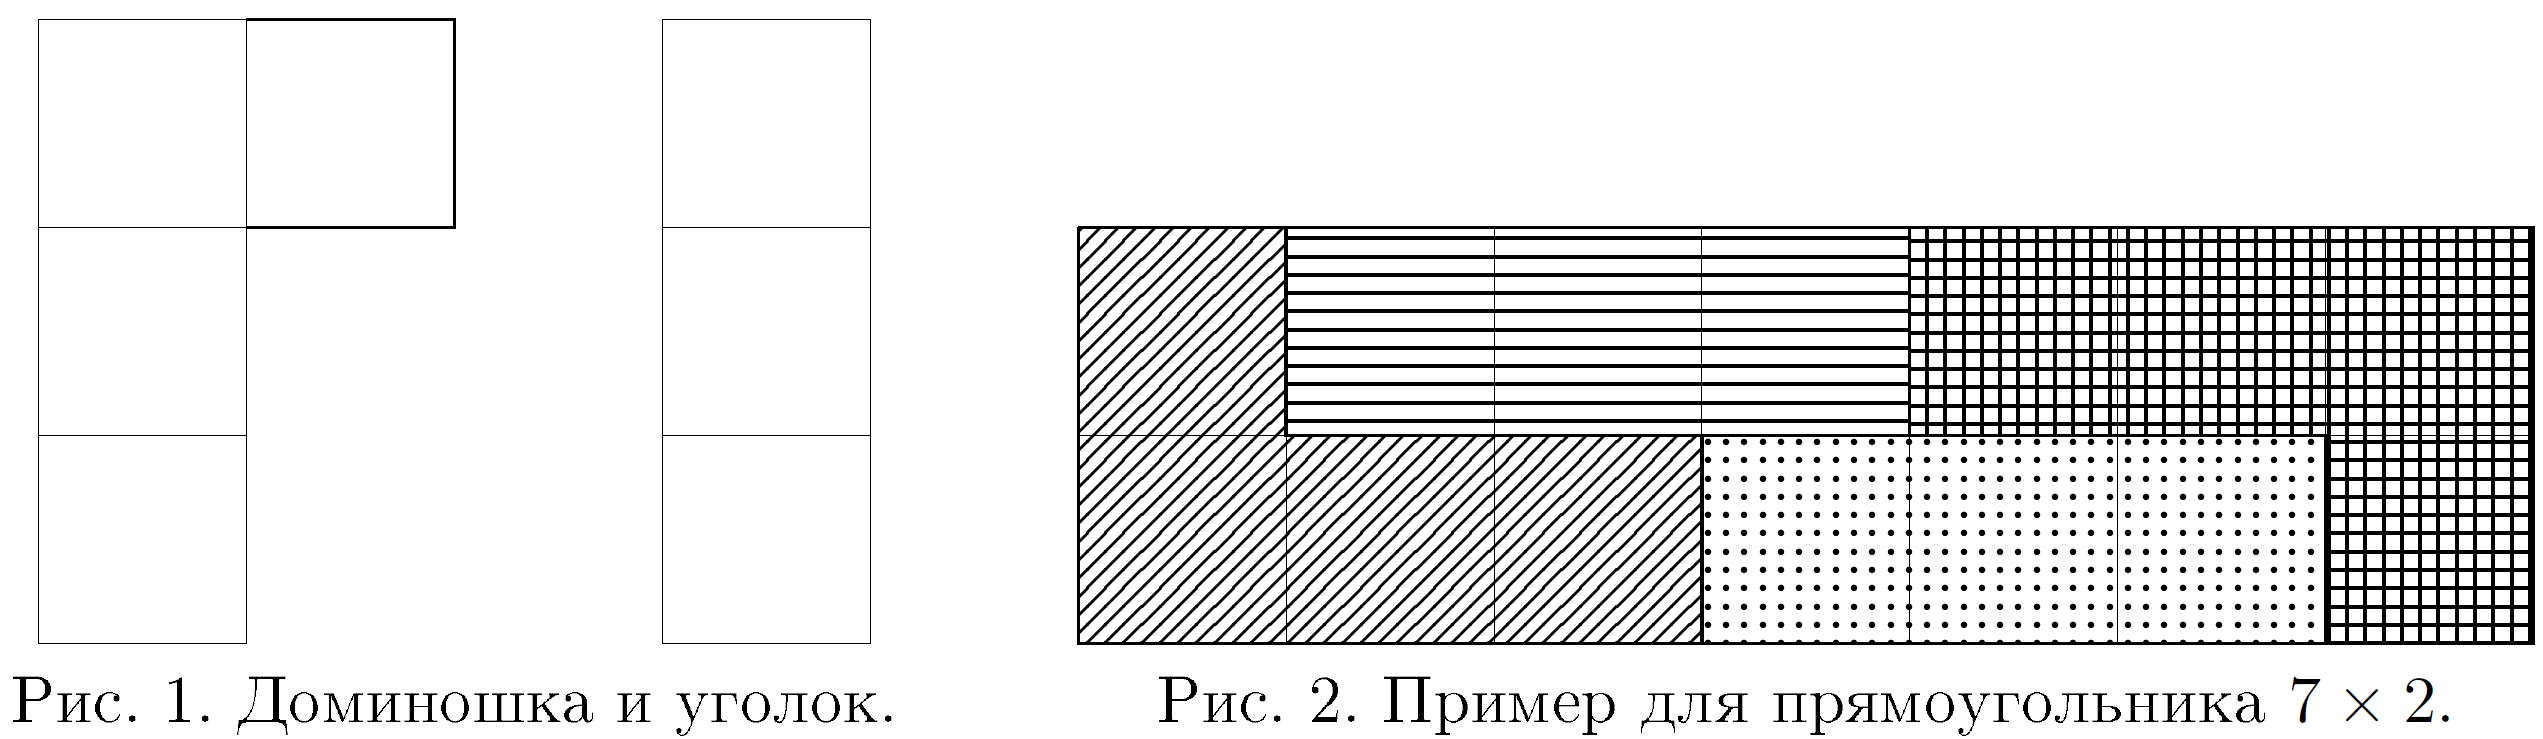
\includegraphics[width=0.65\linewidth]{307_1}
\end{center}
\end{task}

\begin{solution}
Положим в левый верхний угол фигурку и рассмотрим дальнейшие варианты замощения.
\begin{center}
  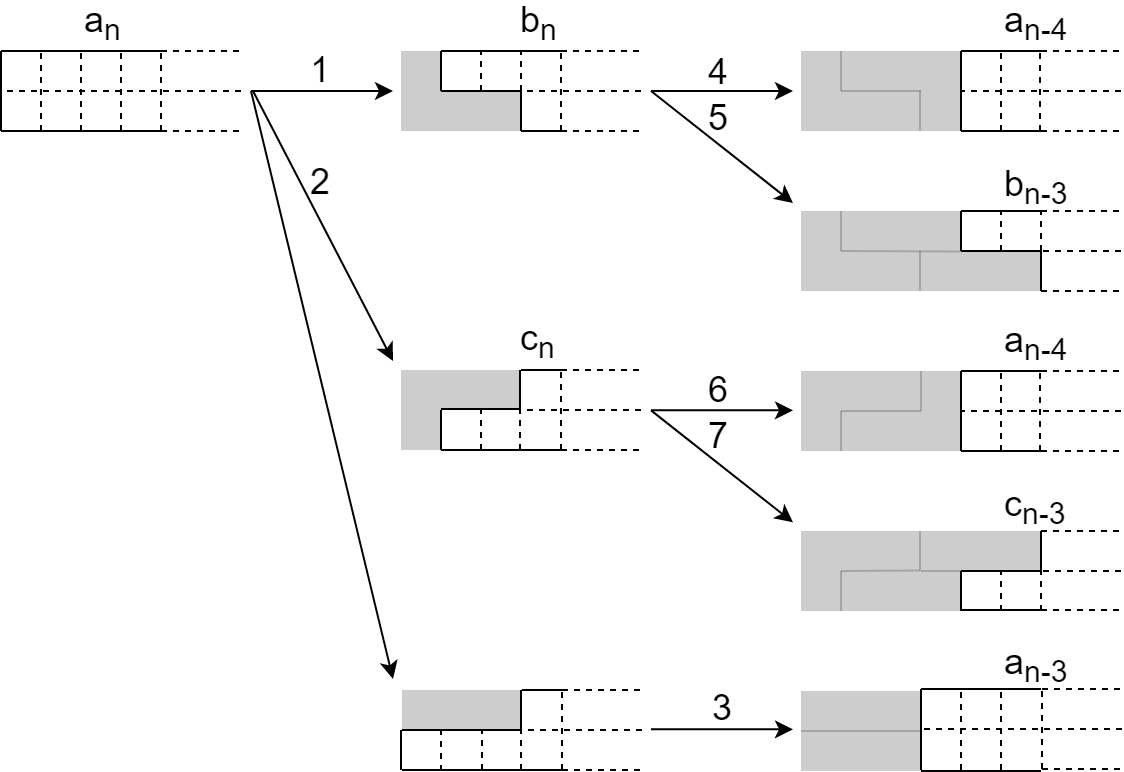
\includegraphics[width=0.65\linewidth]{307_2}
\end{center}
Составим систему уравнений, опираясь на переходы, отмеченные на схеме.
\[
\begin{cases}
    a_n=b_n+c_n+a_{n-3} &\text{из 1, 2 и 3}\\
    b_n =a_{n-4}+b_{n-3} &\text{из 4 и 5}\\
    c_n =a_{n-4}+c_{n-3} &\text{из 6 и 7}
\end{cases}
\]
Решая систему уравнений, получим:
\[a_n=2a_{n-3}+2a_{n-4}-a_{n-6}.\]
$a_0=1$ -- по условию.\\
Простым перебором найдём $a_1 \dots a_6.$\\
$a_1=0\\
a_2=0\\
a_3=1\\
a_4=2\\
a_5=0\\
a_6=1\\$
\end{solution}